\begin{subfigure}[t]{0.32\columnwidth}
    \centering
    \resizebox{\columnwidth}{!}{
        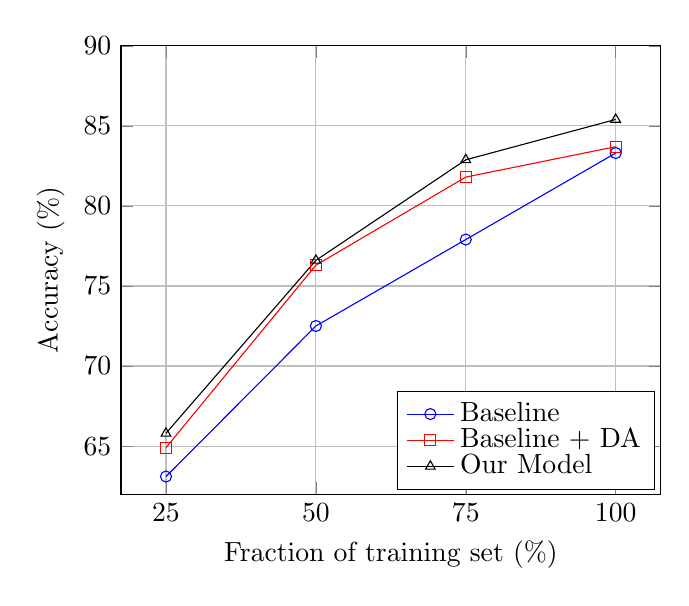
\begin{tikzpicture}[scale=1.0]
          % \footnotesize
          \begin{axis}[ 
            legend cell align={left},
            legend style={legend style={row sep=-3pt},
            at={(0.99,0.01)},anchor=south east},
            % width=1.0\linewidth,
            % height=0.9\linewidth,
            xlabel=Fraction of training set (\%),
            ylabel=Accuracy (\%),
            grid=major,
            % legend pos=south east,
            xlabel near ticks,
            xticklabel style={/pgf/number format/1000 sep=},
            ylabel near ticks,
            xtick=data,
            yticklabel style={
                left,
                /pgf/number format/.cd,
                fixed,
                precision=2,
                /tikz/.cd
            },
            % enlarge y limits={value=.1,upper},
            log ticks with fixed point,
            ymin=62,
            ymax=90,
            cycle list name=color
          ] 
            % \addplot[color=orange,mark=o, mark options={scale=0.5}] coordinates { (10,52.4) (25, 63.1) (50,72.5) (75,77.9) (100,83.3)};
            % \addplot[color=red,mark=o, mark options={scale=0.5}] coordinates { (10,50.3) (25,64.9) (50,76.3) (75,81.8) (100,83.7)};
            % \addplot[color=green,mark=o, mark options={scale=0.5}] coordinates { (10,51.1) (25,65.8) (50,76.6) (75,82.88) (100,85.4)};
            \addplot[color=blue,mark=o] coordinates { (25, 63.1) (50,72.5) (75,77.9) (100,83.3)};
            \addplot[color=red,mark=square] coordinates { (25,64.9) (50,76.3) (75,81.8) (100,83.7)};
            \addplot[color=black,mark=triangle] coordinates { (25,65.8) (50,76.6) (75,82.88) (100,85.4)};                    
            \legend{Baseline, Baseline + DA, Our Model}
          \end{axis}
        \end{tikzpicture}
    }
    \caption{Only geometric transformations}
    \label{fig_BACH_geo}
\end{subfigure}